% ------------------------------------------------------------------------------
% TYPO3 v9 LTS - What's New (English Version)
%
% @author	Michael Schams <schams.net>
% @license	Creative Commons BY-NC-SA 3.0
% @link		https://typo3.org/help/documentation/whats-new/
% @language	English
% ------------------------------------------------------------------------------

\section{Search Engine Optimization}
\begin{frame}[fragile]
	\frametitle{Search Engine Optimization}

	\begin{center}\huge{\color{typo3darkgrey}\textbf{Search Engine Optimization}}\end{center}
	\begin{center}\large{\textit{Now we can "SEO" you}}\end{center}

\end{frame}

% ------------------------------------------------------------------------------

\begin{frame}[fragile]
	\frametitle{Search Engine Optimization}
	\framesubtitle{Search Engine Optimization}

	Page properties feature a new "SEO" tab, which allows BE users to configure
	SEO-related information, \href{http://ogp.me/}{Open Graph} data and much more.

	\begin{figure}
		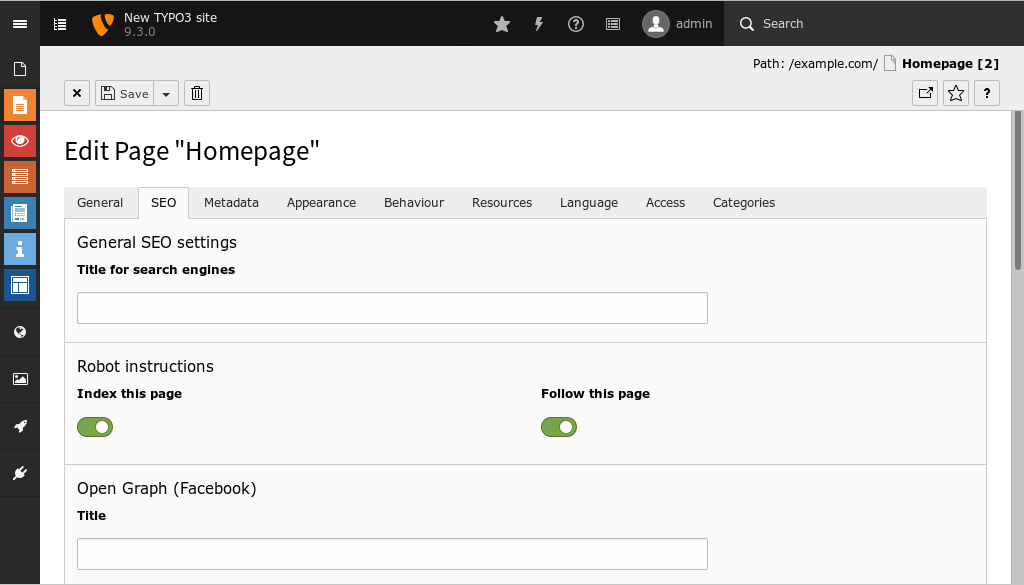
\includegraphics[width=0.70\linewidth]{SearchEngineOptimization/SearchEngineOptimizationPageProperties.png}
	\end{figure}

\end{frame}

% ------------------------------------------------------------------------------

\begin{frame}[fragile]
	\frametitle{Search Engine Optimization}
	\framesubtitle{Search Engine Optimization (SEO)}

	\begin{itemize}
		\item New
			\href{https://docs.typo3.org/typo3cms/CoreApiReference/ApiOverview/PageTitleApi/Index.html}{Page Title API}
			allows integrators and developers to influence what exactly is shown
			as the page title
		\item TYPO3 can generate
			\href{https://docs.typo3.org/typo3cms/CoreApiReference/ApiOverview/XmlSitemap/Index.html}{XML Sitemaps}
			now, with the capability to render different sitemaps per site and
			language
		\item Canonical links to pages are automatically added to prevent
			ranking penalties due to duplicate content for example
		\item In multi-language TYPO3 sites, \texttt{hreflang}-tags are added
			automatically
		\item SEO-related meta tags set in the page properties are now rendered
			in the frontend by default

	\end{itemize}

\end{frame}

% ------------------------------------------------------------------------------
% Meta Tag Manager (API)
% #81464 - Add API for meta tag management

\begin{frame}[fragile]
	\frametitle{Search Engine Optimization}
	\framesubtitle{Meta Tag Manager}

	% decrease font size for code listing
	\lstset{basicstyle=\tiny\ttfamily}

	\begin{itemize}
		\item New
			\href{https://docs.typo3.org/typo3cms/CoreApiReference/ApiOverview/MetaTagApi/Index.html}{Meta Tag API}
			has been introduced to manage and render meta tags in a simple and
			flexible way
		\item TYPO3 core ships an \href{http://ogp.me/}{Open Graph}
			Meta Tag Manager, for example:

\begin{lstlisting}
use \TYPO3\CMS\Core\MetaTag\MetaTagManagerRegistry;
$metaTagManager = MetaTagManagerRegistry::getInstance()->getManagerForProperty('og:title');
$metaTagManager->addProperty('og:title', 'This is the OG title from a controller');
\end{lstlisting}

		\item Functions available include:

			\begin{itemize}
				\smaller
					\item \texttt{\$metaTagManager->addProperty()}
					\item \texttt{\$metaTagManager->removeProperty()}
					\item \texttt{\$metaTagManager->removeAllProperties()}
			\end{itemize}

	\end{itemize}

\end{frame}

% ------------------------------------------------------------------------------
% Meta Tag Manager (API)
% #81464 - Add API for meta tag management

\begin{frame}[fragile]
	\frametitle{Search Engine Optimization}
	\framesubtitle{Meta Tag Manager}

	% decrease font size for code listing
	\lstset{basicstyle=\tiny\ttfamily}

	\begin{itemize}
		\item Developers can register custom \texttt{MetaTagManager} in the
			\texttt{MetaTagManagerRegistry}

\begin{lstlisting}
use \TYPO3\CMS\Core\MetaTag\MetaTagManagerRegistry;
$metaTagManagerRegistry = MetaTagManagerRegistry::getInstance();
$metaTagManagerRegistry->registerManager(
  'custom',
  \Some\CustomExtension\MetaTag\CustomMetaTagManager::class
);
\end{lstlisting}

		\item Meta tags can be set by TypoScript and PHP

\begin{lstlisting}
page.meta {
  og:site_name = TYPO3
  og:site_name.attribute = property
  og:site_name.replace = 1
}
\end{lstlisting}

			\smaller
				("\texttt{replace = 1}" replaces earlier set meta tags)
			\normalsize

	\end{itemize}

\end{frame}

% ------------------------------------------------------------------------------
